\newcommand{\FigPhaseII}{
\begin{figure}[t]
\centering
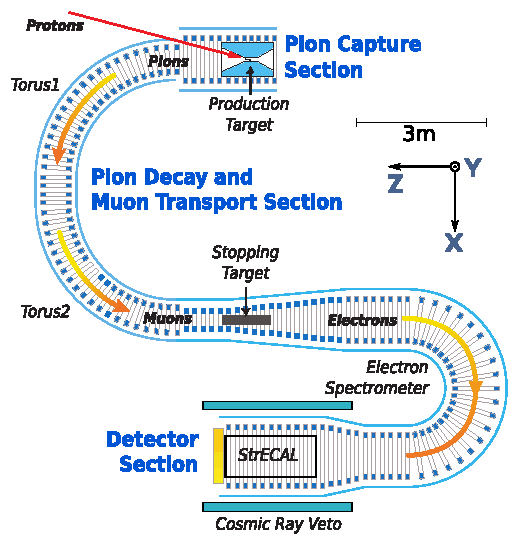
\includegraphics[width=0.9\textwidth]{figs/detector/PhaseII_schematic}
\caption{
Schematic layout of COMET \phaseII. 
The 8 GeV proton beam enters from the top-left, producing (amongst other things) pions.
Pions and muons travelling backwards with respect to the proton beam are then transported around 180 degrees of bent solenoid, during which time most of the pions decay producing an intense muon beam.
About 40\% of these muons then stop in the stopping target (centre of image).
Any electrons coming from  \mueconv are then transported through another 180 degrees of bent solenoid into the detector system.
}
\label{detector:PhaseII:setup}
\end{figure}
}

\newcommand{\FigPhaseI}{
\begin{figure}[t]
\centering
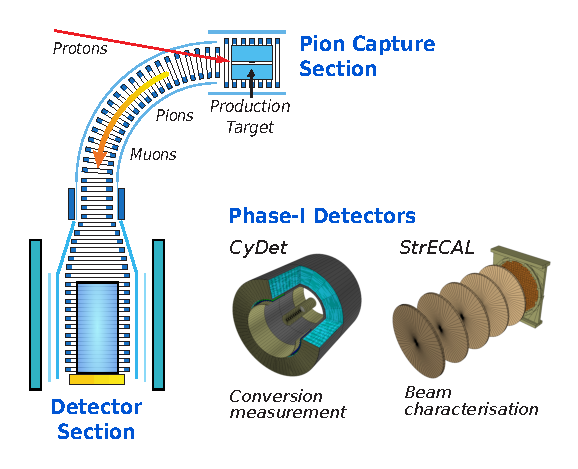
\includegraphics[height=0.4\textheight]{figs/detector/PhaseI_schematic}
\caption{
Schematic layout of COMET \phaseI. 
}
\label{detector:PhaseI:setup}
\end{figure}
}
